\tikzset{%
  % Specifications for style of nodes:
         base/.style = {rectangle, rounded corners, draw = black, minimum width=2.5cm, minimum height=1cm, fill=orange!15, font=\ttfamily},
}

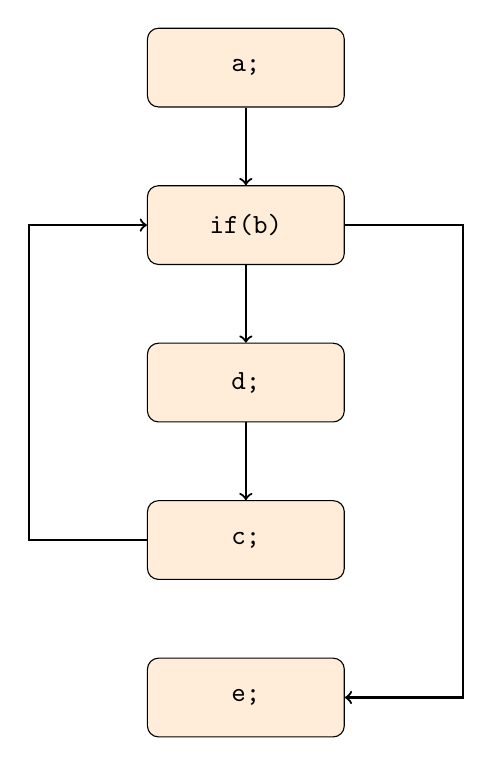
\begin{tikzpicture}[node distance=2cm, every node/.style={fill=white, font=\sffamily}, align=center]
    % Draw nodes
    \node (start)       [base]                        {a;};
    \node (if)          [base, below of = start]      {if(b)};
    \node (code)        [base, below of = if]         {d;};
    \node (incr)        [base, below of = code]       {c;};
    \node (end)         [base, below of = incr]       {e;};

    % Draw arrows
    \draw[->,thick]           (start) -- (if);
    \draw[->,thick]              (if) -- (code);
    \draw[->,thick]            (code) -- (incr);

    \draw[->,thick]            (incr.west) -- ++(-1.5,0) -- ++(0,4) -- ++(1.5,0) (if);
    \draw[->,thick]         (if.east) -- ++(1.5,0) -- ++(0,-6) -- ++(-1.5,0)     (end);


\end{tikzpicture}
